\documentclass[french]{standalone}
\usepackage{babel}
\usepackage{tkz-fct}
\usepackage{tkz-euclide}
\usepackage{color}
\usepackage{amsmath}
\usepackage{numprint}
\usepackage{amssymb}
\usepackage{amsthm}
\renewcommand*\familydefault{\sfdefault}
\usepackage{sansmath}
\sansmath
\definecolor{gray75}{gray}{0.75}
\usepackage{setspace}
	\setstretch{1.25}
\begin{document}
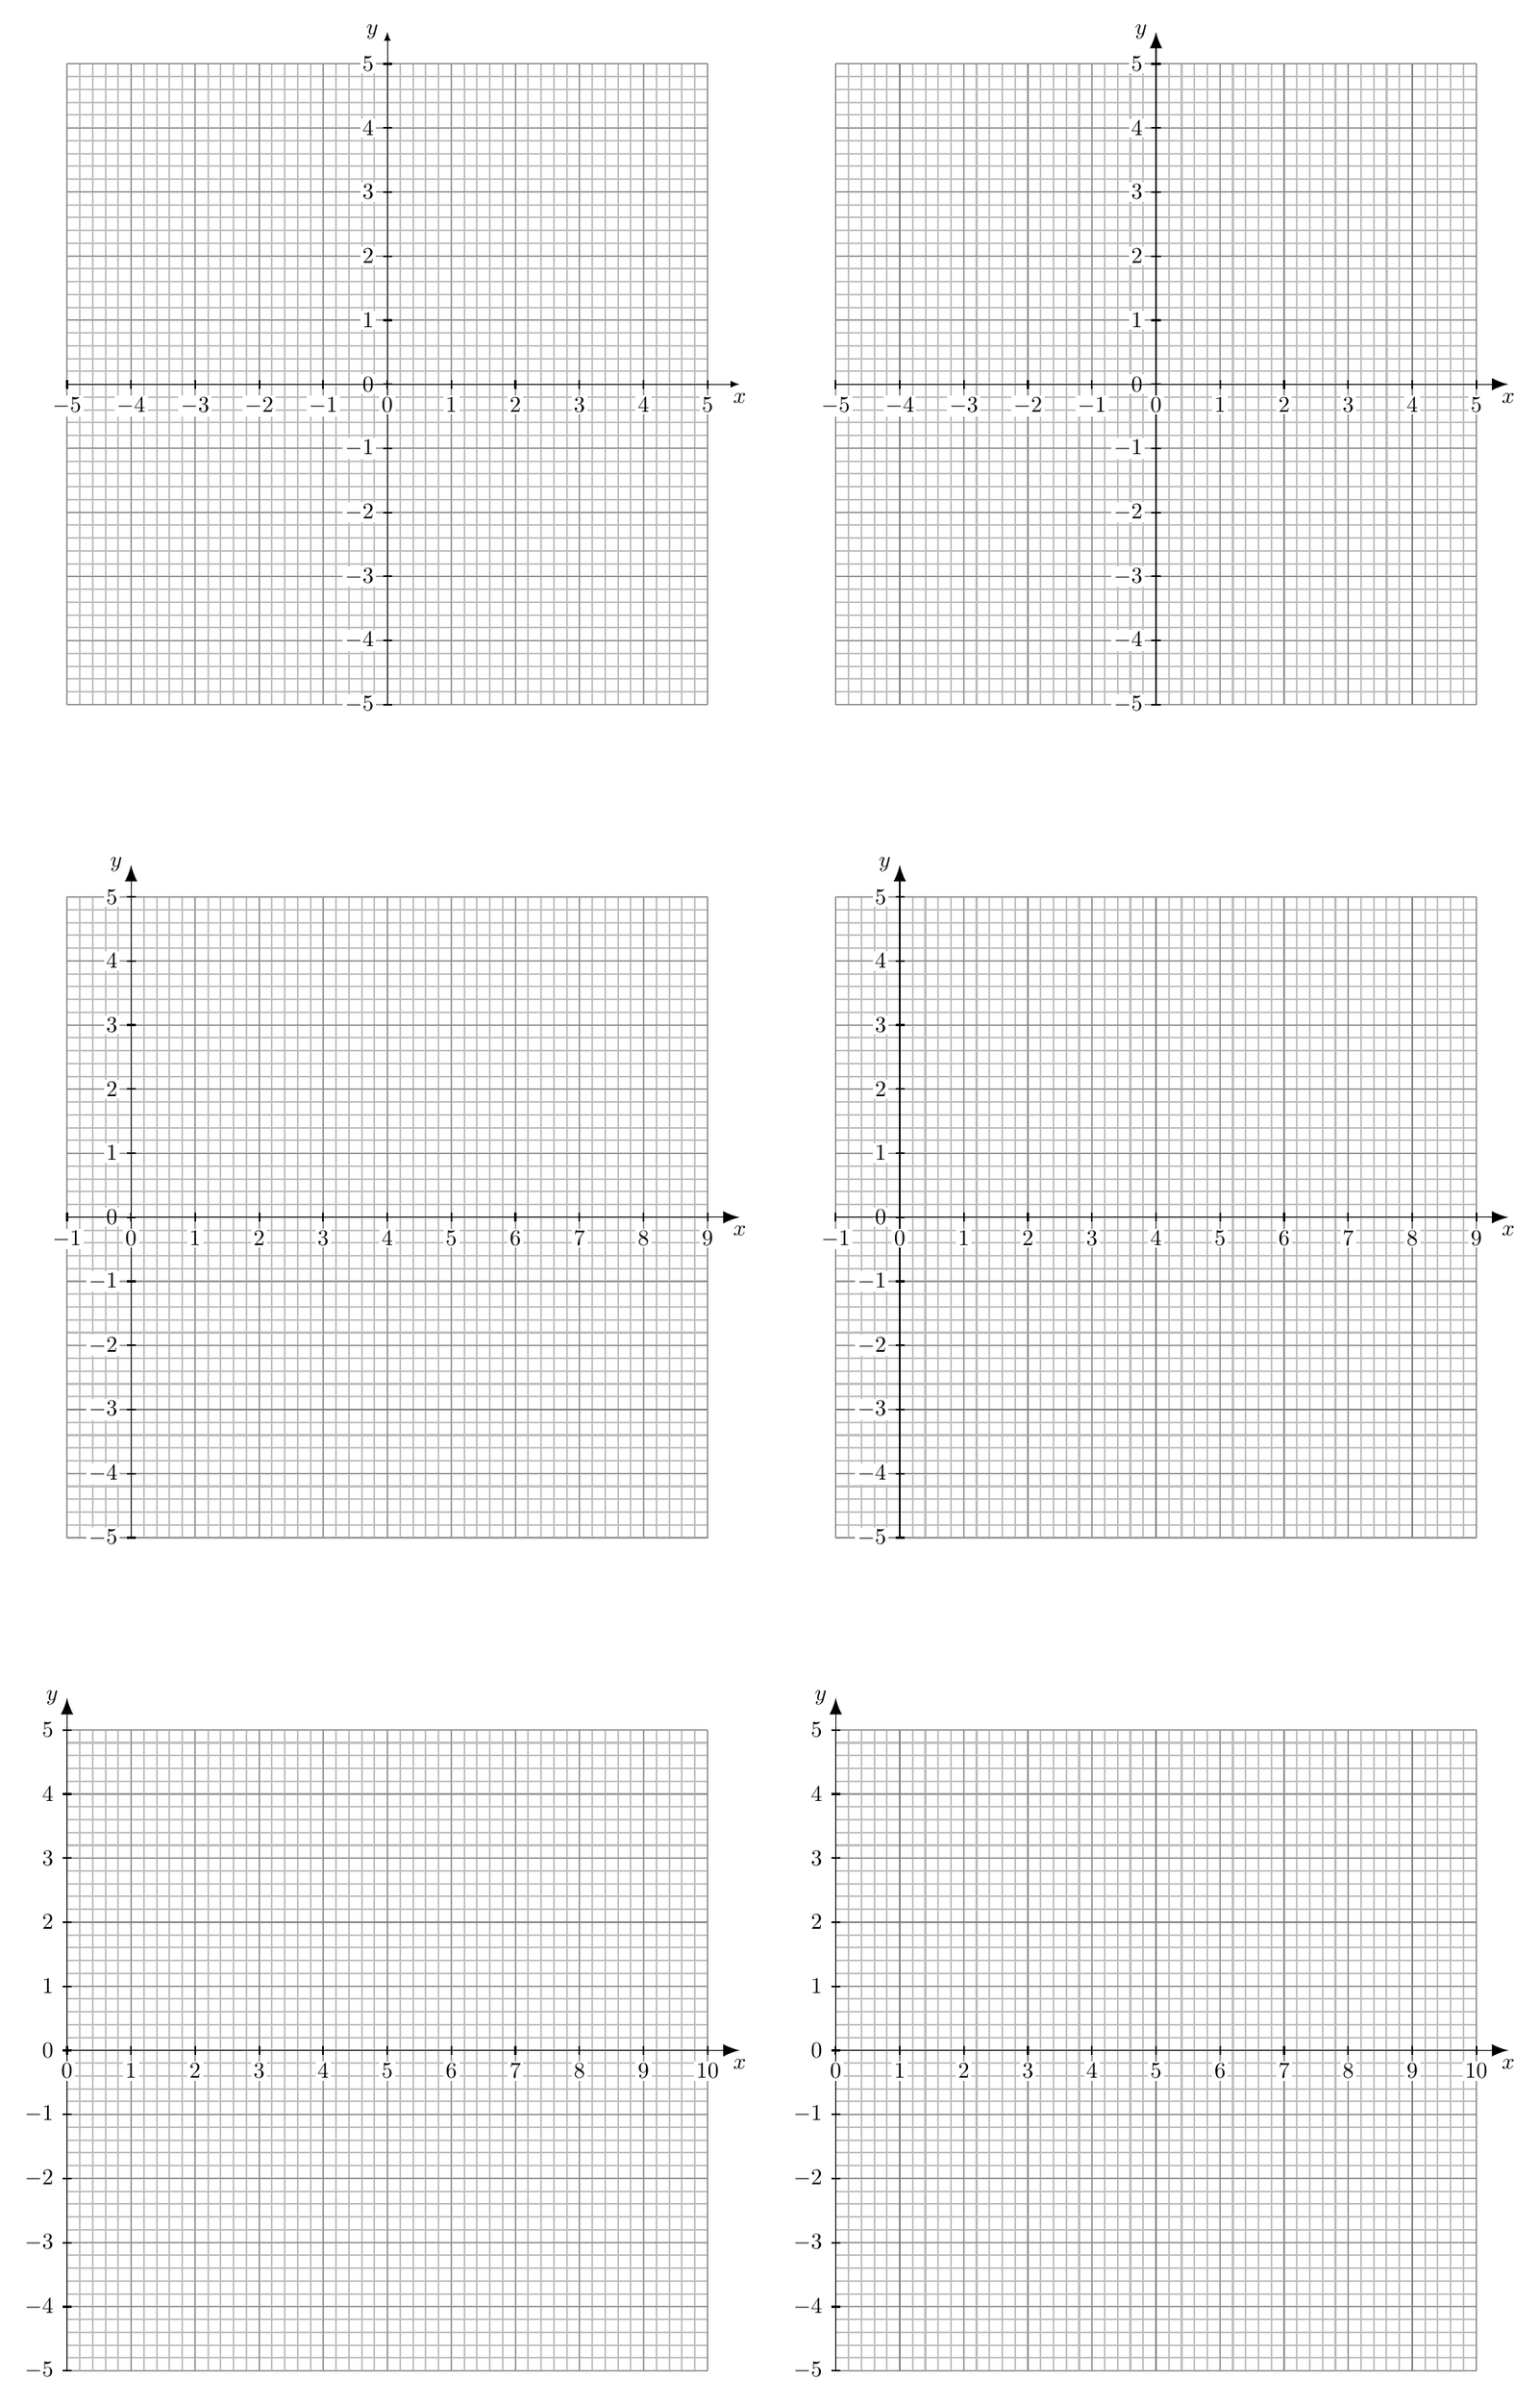
\begin{tikzpicture}
  \tkzInit[xmin=-5,xmax=5,ymin=-5,ymax=5, ystep=1, xstep=1]

     \begin{scope}
     \tkzGrid[color=gray,sub,subxstep=0.2, subystep=0.2]
   \end{scope}
\tkzAxeY
\tkzDrawX
\tkzLabelX
\tkzFct[domain=-5:5,line width=1.5pt]{(1/exp(x))}


\begin{scope}[xshift=12cm]
  \tkzInit[xmin=-5,xmax=5,ymin=-5,ymax=5, ystep=1, xstep=1]

     \begin{scope}
     \tkzGrid[color=gray,sub,subxstep=0.2, subystep=0.2]
   \end{scope}
\tkzAxeY
\tkzDrawX
\tkzLabelX
\tkzFct[domain=-5:2,line width=1.5pt]{(exp(log(4)*x))}

\end{scope}
\begin{scope}[yshift=-13cm, xshift=-4cm]
  \tkzInit[xmin=-1,xmax=9,ymin=-5,ymax=5, ystep=1, xstep=1]

     \begin{scope}
     \tkzGrid[color=gray,sub,subxstep=0.2, subystep=0.2]
   \end{scope}
\tkzAxeY
\tkzDrawX
\tkzLabelX
\tkzFct[domain=0.001:10,line width=1.5pt]{(log(\x)/log(0.5))}


\begin{scope}[xshift=12cm]
  \tkzInit[xmin=-1,xmax=9,ymin=-5,ymax=5, ystep=1, xstep=1]

     \begin{scope}
     \tkzGrid[color=gray,sub,subxstep=0.2, subystep=0.2]
   \end{scope}
\tkzAxeY
\tkzDrawX
\tkzLabelX
\tkzFct[domain=0.001:10,line width=1.5pt]{(log(\x)/log(5))}


\end{scope}
\end{scope}  
\begin{scope}[yshift=-26cm, xshift=-5cm]
  \tkzInit[xmin=0,xmax=10,ymin=-5,ymax=5, ystep=1, xstep=1]

     \begin{scope}
     \tkzGrid[color=gray,sub,subxstep=0.2, subystep=0.2]
   \end{scope}
\tkzAxeY
\tkzDrawX
\tkzLabelX
\tkzFct[domain=0.00001:10,line width=1.5pt]{(log(\x)/log(10))}


\begin{scope}[xshift=12cm]
  \tkzInit[xmin=0,xmax=10,ymin=-5,ymax=5, ystep=1, xstep=1]

     \begin{scope}
     \tkzGrid[color=gray,sub,subxstep=0.2, subystep=0.2]
   \end{scope}
\tkzAxeY
\tkzDrawX
\tkzLabelX
\tkzFct[domain=0.00001:10,line width=1.5pt]{(-log(\x)/log(10))}


\end{scope}
\end{scope} 
\end{tikzpicture}
\end{document}
